\documentclass[
coverheight=9in,
coverwidth=6in,
spinewidth=0.756in,
bleedwidth=.125in,
marklength=0in,
markcolor=black]{bookcover}
\usepackage[T1]{fontenc}
\usepackage[russian]{babel}


\newbookcoverpart{pback}{
\setpartposx{\marklength+\bleedwidth+10mm}
\setpartposy{\marklength+\bleedwidth+10mm}\setpartheight{\coverheight-20mm}
\setpartwidth{\coverwidth-20mm}
\settrimmedpart{0mm}{0mm}{0pt}{0pt}
}

\begin{document}

\begin{bookcover}

\definecolor{mycolor}{HTML}{a2521d}
\bookcovercomponent{color}{bg whole}{mycolor}

\bookcovercomponent{center}{front}{
\vskip-.125in
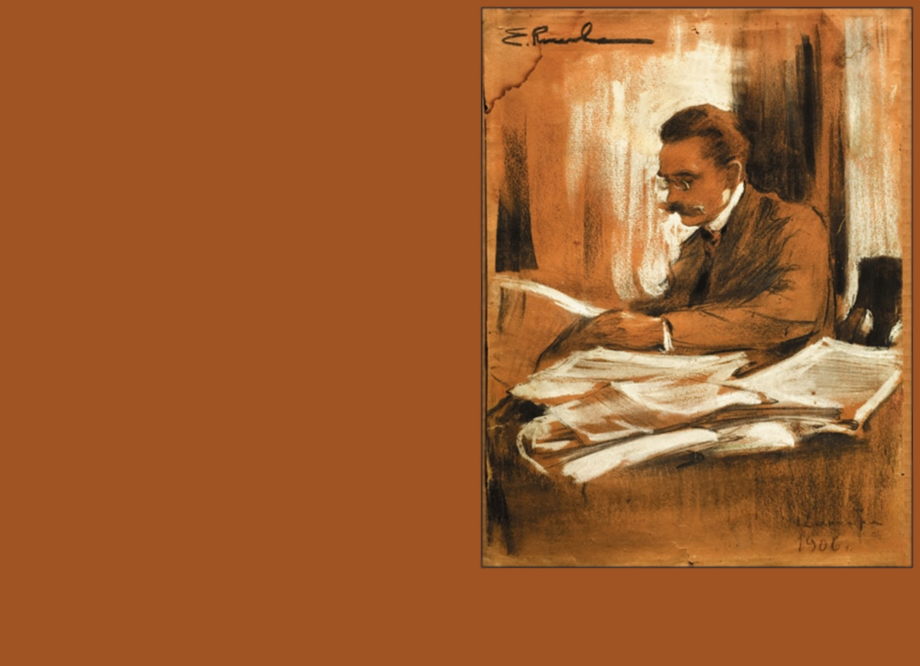
\includegraphics[width=\textwidth]{kiselyov}
\vfill
\color{yellow!10}\fontsize{28}{48}\usefont{T2A}{cmr}{b}{n} ГЕОМЕТРИЯ ПО КИСЕЛЁВУ
\vskip10mm
}

\bookcovercomponent{center}{spine}
{\rotatebox[origin=c]{90}{\color{yellow!10}\fontsize{20}{48}\usefont{T2A}{cmr}{b}{n}  ГЕОМЕТРИЯ ПО КИСЕЛЁВУ}}


\bookcovercomponent{center}{pback}{
\begin{flushleft}
\parbox{.7\textwidth}{
\color{yellow!10}\fontsize{12}{10}\usefont{T2A}{cmr}{b}{n}Издание классического школьного учебника по геометрии. За основу взято издание 1938 года, но использовались также издания 1914 и 1931 годов.
}
\end{flushleft}
\vfill
{
\color{yellow!10}\fontsize{14}{10}\texttt{anton-petrunin.github.io/kiselyov}}
\hfill\includegraphics{978-1-68474-812-9}
}

\end{bookcover}

\end{document}
